\documentclass[12pt]{article}
\usepackage{amsmath}
\usepackage{graphicx}
\usepackage{float}
\usepackage{listings}
\usepackage{xcolor}

% Ajustes de estilo
\definecolor{titlecolor}{RGB}{30, 97, 183}
\definecolor{subtitlecolor}{RGB}{49, 130, 189}
\definecolor{sectioncolor}{RGB}{0, 102, 51}
\definecolor{subsubsectioncolor}{RGB}{153, 0, 0}
\definecolor{codecolor}{RGB}{102, 102, 102}

\usepackage[margin=2.5cm]{geometry}

\begin{document}
%el documento consiste en una introduccion a el robot gekko, como interactuar con el y como programarlo
\title{\textcolor{titlecolor}{Robot GEKKO}}
\author{Team Mustabot 2022}
\date{\today}
%ahora introducimos los componentes del robot
\maketitle

\section*{\textcolor{sectioncolor}{Componentes Principales}}
%&subtitulo
\subsection*{\textcolor{subtitlecolor}{Sensores}}
%aca explicamos los sensores
%subtitulo dentro del subtitulo
\subsubsection*{\textcolor{subsubsectioncolor}{Infrarrojos}}
Gekko posee un total de 8 sensores infrarrojos, los cuales son utilizados para seguir líneas negras y blancas.
Estos están colocados de manera que cuando el robot se encuentre en movimiento, tengan un ángulo de 90 grados respecto
a la línea que se desea seguir, esto es para que el robot pueda detectar la línea en todo momento.

%añadimos una imagen del sensor
\begin{figure}[H]
    \centering
    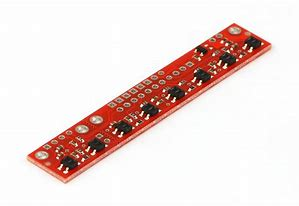
\includegraphics[width=0.5\textwidth]{sensor_images/infrarrojo.jpeg}
    \caption{Sensor Infrarrojo}
    \label{fig:sensor_infrarrojo}
\end{figure}

Para acceder a los valores del sensor infrarrojo, llamamos a la función \texttt{get\_infrarrojo} y el índice del sensor, están enumerados del 0 al 7 de izquierda
a derecha.

%ejemplo del codigo
\begin{lstlisting}[language=C++, basicstyle=\color{codecolor}]
    //definimos los pines del robot
    void setup(){
        //inicializamos los sensores infrarrojos
        infrarrojo_init();
    }
    void loop(){
        //leemos el sensor infrarrojo 1
        infrarrojo_1 = get_infrarrojo(1);
        Serial.println(infrarrojo_1);
        //leemos el sensor infrarrojo 2
        infrarrojo_2 = get_infrarrojo(2);
        Serial.println(infrarrojo_2);
    }
\end{lstlisting}

\subsubsection*{\textcolor{subsubsectioncolor}{Laser}}
Para efectos de detectar los obstáculos que se presentan en el camino, el robot posee 5 sensores Laser, los cuales
emiten una luz en línea recta, la cual es reflejada por los objetos que se encuentran en el camino. Estos sensores permiten
detectar la distancia del objeto que se presenta en el camino, además no tienen problemas con la luz del sol ni con el color
que presenten los obstáculos.

%añadimos una imagen del sensor
\begin{figure}[H]
    \centering
    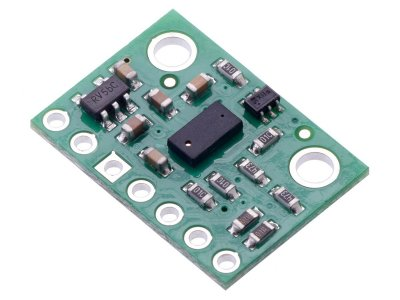
\includegraphics[width=0.5\textwidth]{sensor_images/laser.jpeg}
    \caption{Sensor Laser}
    \label{fig:sensor_laser}
\end{figure}

Para obtener el valor del sensor laser, debemos usar la función \texttt{get\_laser}, la cual recibe como input el índice del sensor que queremos obtener.

%ejemplo del codigo
\begin{lstlisting}[language=C++, basicstyle=\color{codecolor}]
    //definimos los pines del robot
    void setup(){
        //inicializamos los sensores laser
        laser_init();
    }
    void loop(){
        //leemos el sensor laser 1
        laser_1 = get_laser(1);
        Serial.println(laser_1);
        //leemos el sensor laser 2
        laser_2 = get_laser(2);
        Serial.println(laser_2);
    }
\end{lstlisting}

\subsubsection*{\textcolor{subsubsectioncolor}{Color}}
Cuando se nos presentan colores en la pista, estos siempre se encuentran en una posición relativa específica, por esta razón, los sensores de color
se encuentran fijos detrás de los sensores infrarrojos. Estos sensores nos permitirán detectar el total de luz ambiente y el porcentaje de cada componente
RGB que presenta la luz.

%añadimos una imagen del sensor
\begin{figure}[H]
    \centering
    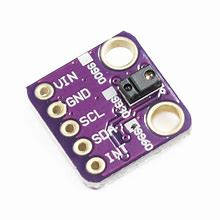
\includegraphics[width=0.5\textwidth]{sensor_images/color.jpeg}
    \caption{Sensor Color}
    \label{fig:sensor_color}
\end{figure}

Para acceder a los valores del sensor de color, usamos la función \texttt{get\_color}, la cual recibe como parámetro el número del sensor de color que se desea leer,
1 el derecho y 0 el izquierdo.

\begin{lstlisting}[language=C++, basicstyle=\color{codecolor}]
    //definimos los pines del robot
    void setup(){
        //inicializamos los sensores de color
        color_init();
    }
    void loop(){
        //leemos el sensor de color derecho
        color_derecho = get_color(1);
        Serial.println(color_derecho);
        //leemos el sensor de color izquierdo
        color_izquierdo = get_color(0);
        Serial.println(color_izquierdo);
    }
\end{lstlisting}

\subsection*{\textcolor{subtitlecolor}{Motores}}
%aca explicamos los motores
El robot posee 2 motores, dispuestos en sentido opuesto y en la parte delantera del mismo. Estos motores son los encargados de mover el robot, hacerlo girar
y detenerlo.

%añadimos una imagen del motor
\begin{figure}[H]
    \centering
    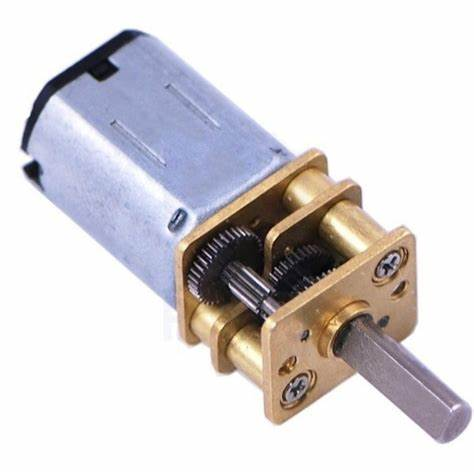
\includegraphics[width=0.5\textwidth]{actuador_images/motor.jpeg}
    \caption{Motor}
    \label{fig:motor}
\end{figure}

Los motores son controlados mediante potencia, es decir, mediante el código suministramos un valor de potencia que pertenezca al intervalo [0,255]. Para
esto, usamos la función \texttt{mov}, la cual recibe como parámetros la potencia del motor izquierdo y la potencia del motor derecho respectivamente.

\begin{lstlisting}[language=C++, basicstyle=\color{codecolor}]
    void setup(){
        motor_init();
    }
    void loop(){
        mov(255,255);
        delay(1000);
        mov(-255,-255);
        delay(1000);
    }
\end{lstlisting}

\subsection*{\textcolor{subtitlecolor}{Física del Movimiento}}
El robot posee tracción delantera, es decir, los motores se encuentran en la parte delantera del robot, esto nos permite que el robot pueda girar sobre sí mismo
al tener un roce muy pequeño en la parte trasera, por ende una resistencia muy pequeña al momento de girar.
Esto trae consigo algunos problemas, como la tracción al momento de subir, el cual se soluciona colocando el centro de masa del robot dentro del eje de las
ruedas que poseen tracción, en este caso las ruedas delanteras.

\begin{figure}[H]
    \centering
    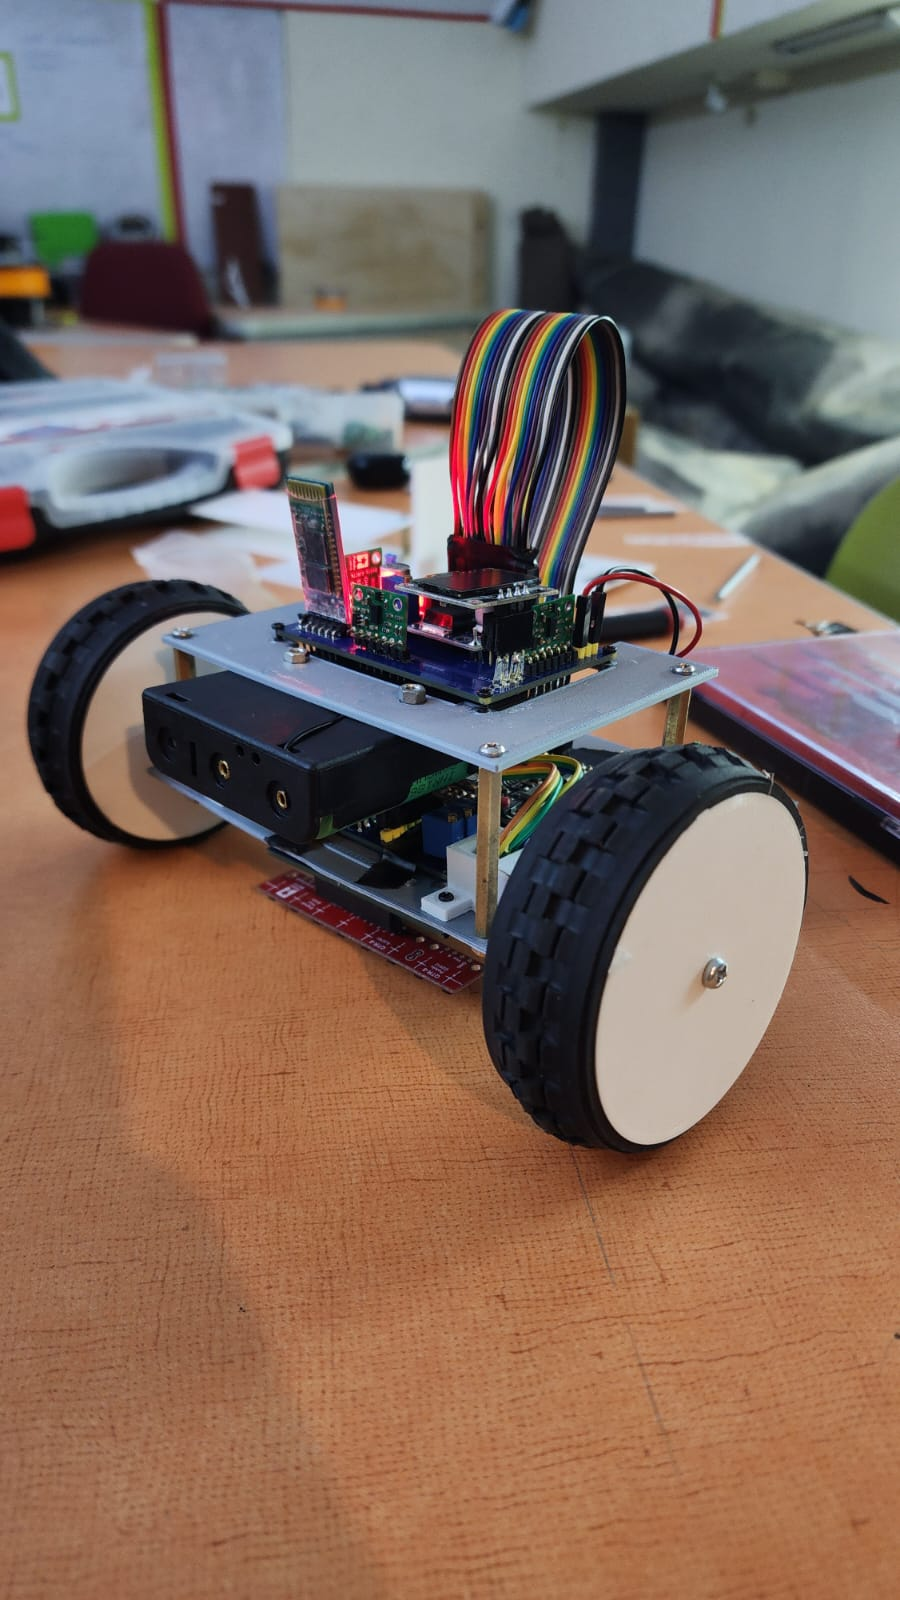
\includegraphics[width=0.5\textwidth]{robot_images/robot1.jpeg}
    \caption{Robot}
    \label{fig:robot}
\end{figure}
%añadimos una imagen del robot
%\begin{figure}[H]
%    \centering
%    \includegraphics[width=0.5\textwidth]{robot_images/robot.jpeg}
%    \caption{Robot}
%    \label{fig:robot}
%\end{figure}

\subsection*{\textcolor{subtitlecolor}{Desafío}}
Realicen un debug de los sensores del robot, para esto deben usar la comunicación serial, la cual les permitirá
conseguir los datos del robot, apóyense en las funciones antes vistas.
\end{document}